%\documentclass[handout,t,xcolor=pdftex,dvipsnames,table]{beamer}
\documentclass[t,xcolor=pdftex,dvipsnames,table]{beamer}
\title[ST-SMM]{Symptom Tracker using Social Media Messaging --- {\small for users with limited internet } } 
\usepackage{beamerthemesplit}%headline and footline split in two parts
\usepackage{rotating}
\usepackage{refstrings}
\usepackage{listings}
%\usepackage{pgf}


\usepackage{calc}
\usepackage{environ}

\newcommand{\halfmargin}{0.01\paperwidth}
%\newcommand{\margin}{0.10\paperwidth}

%\beamersetrightmargin{\margin}
%\beamersetleftmargin{\margin}

\NewEnviron{wideframe}[1][]{%
  \begin{frame}{#1}
    \makebox[\textwidth][c]{
      \begin{minipage}{\dimexpr\paperwidth-\halfmargin-\halfmargin\relax}
        \BODY
      \end{minipage}}
  \end{frame}
}




\usetheme{Szeged}
% AnnArbor Antibes Bergen Berkeley Berlin Boadilla boxes 
% CambridgeUS Copenhagen Darmstadt default Dresden Frankfurt 
% Goettingen Hannover Ilmenau JuanLesPins Luebeck Madrid 
% Malmoe Marburg Montpellier PaloAlto Pittsburgh Rochester 
% Singapore Szeged Warsaw

%\setbeamercovered{transparent}
% or whatever (possibly just delete it)

\usecolortheme{seagull} 
% albatross beaver beetle crane default dolphin 
% dove fly lily orchid rose seagull seahorse 
% sidebartab structure whale wolverine

% classical large headings
\usefonttheme[onlylarge]{structuresmallcapsserif}

% thick navigation font 
\usefonttheme[onlysmall]{structurebold} 

%\setbeamerfont{title}{shape=\itshape,family=\rmfamily}
%\setbeamercolor{title}{fg=red!80!black,bg=red!20!white}

%%%%%%%%%%%%%%%%%%%%%% PACKAGES %%%%%%%%%%%%%%%%%%%%%%%%%%%%%

\usepackage{relsize}
\usepackage{fancyvrb}
\usepackage{xmpmulti}
\usepackage{ifthen}
\usepackage{multirow}

\usepackage[english]{babel}
\usepackage[latin1]{inputenc}

%\usepackage{times}
%\usepackage{bookman}
\usepackage{lmodern}
\usepackage[T1]{fontenc}
%\usepackage[T1]{fontenc}
% Or whatever. Note that the encoding and the font should match. If T1
% does not look nice, try deleting the line with the fontenc.


\RequirePackage{amsmath}
%\RequirePackage{amsthm}
\RequirePackage{amssymb}
%\RequirePackage{latexsym}
\RequirePackage{mathtools}

%\RequirePackage{xspace}
\RequirePackage{url}

%\usepackage[pdftex]{graphicx}

\RequirePackage{color}

%%%%%%%%% logic slides 
\newcommand{\iphi}{{\cal I}(\phi)(\sigma)}
\newcommand{\ipsi}{{\cal I}(\psi)(\sigma)}
\newcommand{\gs}[1]{\ensuremath{\gamma_{\sigma}(#1)}} 
\newcommand{\gss}[2]{\ensuremath{\gamma_{\sigma_{#1}}(#2)}} 

%%%%%%%%%%%%%%%%%%%%%%%%%%% Abbreviations
\newcommand{\assig}{\ensuremath{\sigma}}
\newcommand{\asg}{\ensuremath{\sigma}}
\newcommand{\tf}{\ensuremath{\{\true, \false\}}}
\newcommand{\Fo}{\ensuremath{\mathcal{F}}}
\newcommand{\form}{\ensuremath{\mathit{form}}}
\newcommand{\vphi}{\ensuremath{\varphi}}

\newcommand{\valpha}{\ensuremath{\mathit{alpha}}}
\newcommand{\numeric}{\ensuremath{\mathit{numeric}}}
\newcommand{\wspace}{\ensuremath{\mathit{wspace}}}
\newcommand{\vnewline}{\ensuremath{\mathit{newline}}}
\newcommand{\blank}{\ensuremath{\mathit{blank}}}
\newcommand{\word}{\ensuremath{\mathit{word}}}
\newcommand{\lline}{\ensuremath{\mathit{line}}}
\newcommand{\para}{\ensuremath{\mathit{para}}}

%%%%%%%%%%%%%%%%%%%%%%%% Lists
\newcommand{\be}{\begin{itemize}}
\newcommand{\ee}{\end{itemize}}
\newcommand{\bdn}{\begin{description}}
\newcommand{\edn}{\end{description}}
\newcommand{\bn}{\begin{enumerate}}
\newcommand{\en}{\end{enumerate}}
\renewcommand{\i}{\item}

\newenvironment{closeitemize}{\begin{list}%
{$\bullet$}%
{\setlength{\itemsep}{-0.2\baselineskip}%
\setlength{\topsep}{0.2\baselineskip}}}%
{\end{list}}




%%%%%%%%%%%%%%%%%%%%%%%%%%%%%% MISC

\newcommand{\remove}[1]{}

%\newcommand{\case}[2]{\vspace{1.5ex} \noindent \textit{Case} #1: \emph{#2}.}
\newcommand{\scase}[2]{\vspace{1.5ex} \noindent \textit{Subcase} #1: #2.}
\newcommand{\sscase}[2]{\vspace{1.0ex} \noindent \textit{Subsubcase} #1: #2.}

%\newcommand{\defn}[1]{\textit{#1}}
\newcommand{\defi}[1]{\textit{#1}:}



%%%%%%%%%%%%%%%%%%%%%%%%%%%% FOOTNOTES AND THEOREMS


%\newtheorem{definition}{Definition}[]
%\newtheorem{theorem}{Theorem}
%\newtheorem{lemma}{Lemma}
%\newtheorem{proposition}{Proposition}
%\newtheorem{corollary}{Corollary}
%\renewcommand{\thefootnote}{\arabic{footnote}}


%%%%%%%%%%%%%%%%%%%%%%%%%%%%%%%%%%% Text
\newcommand{\smpage}{\noindent \parbox{\textwidth}}
\newcommand{\samep}{\parbox{\textwidth}}   % put onto the same page


\newcommand{\mathid}[1]{\ensuremath{\mathit{#1}}\xspace}

\newcommand{\bc}{\begin{center}}
\newcommand{\ec}{\end{center}}
\newcommand{\ul}{\underline}
\newcommand{\bs}{\bigskip}
%\newcommand{\ms}{\medskip}
%\renewcommand{\ss}{\smallskip}

\newcommand{\bfg}{\begin{figure}}
\newcommand{\efg}{\end{figure}}

\renewcommand{\ss}{\smallskip}
\newcommand{\Eg}{E.g.,\xspace}
\newcommand{\eg}{e.g.,\xspace}
\newcommand{\ie}{i.e.,\xspace}


\newcommand{\intr}{\empi}
\newcommand{\intrdef}{\emph}

\newcommand{\emp}[1]{\textbf{#1}}
\newcommand{\empp}[1]{\emph{#1}}
\newcommand{\empb}[1]{\textbf{#1}}
\newcommand{\empi}[1]{\textit{#1}}
\newcommand{\empbi}[1]{\textbf{\textit{#1}}}

\newcommand{\ind}{\hspace*{3.0em}}

%%%%%From Nancy's book directory:  This spaces the symbols within a
%%%%%word nicely, in math mode.
\newcommand{\ms}[1]{%
        \relax\ifmmode
                \mathord{\mathcode`\-="702D\it #1\mathcode`\-="2200}%
        \else
                $\mathord{\mathcode`\-="702D\it #1\mathcode`\-="2200}$%
        \fi
}


\newcommand{\cmnt}{\`}


%%%%%%%%%%%%%%%%%%%%%%% GENERAL MATH SYMBOLS %%%%%%%%%%%%%%%%%%%%%%%%%%%%%%

\newcommand{\Adj}{\mathop{\rm Adj}\nolimits}
\newcommand{\abs}[1]{\left| #1\right|}
\newcommand{\card}[1]{\left| #1\right|}
\newcommand{\ar}{\rightarrow}
%\newcommand{\ar}{\longrightarrow}
\newcommand{\al}{\alpha}
\renewcommand{\b}[1]{\overline{#1}}
\newcommand{\cat}{\mathbin{\frown}}
\newcommand{\choice}{\mbox{$[\hspace*{-1.0pt}]$}}
\newcommand{\ceil}[1]{\left\lceil #1 \right\rceil}
\renewcommand{\d}{\, . \,}      % separator in quantified formulae
\newcommand{\df}{\triangleq}
%\newcommand{\df}{\mbox{$\:\stackrel{\rm df}{=\!\!=}\:$}}
\newcommand{\dn}{\mbox{$\hspace{-0.1em}\downarrow\hspace{-0.1em}$}}
\newcommand{\Ex}{\mathop{\rm Ex}}
\newcommand{\es}{``"}   %empty string
\newcommand{\expect}[1]{{\rm E}\left[ #1 \right]}
\newcommand{\expectsq}[1]{{\rm E}^2\left[ #1 \right]}
\newcommand{\floor}[1]{\left\lfloor #1 \right\rfloor}
\renewcommand{\ge}{\geqslant}
\newcommand{\given}{\mid}
\newcommand{\halfind}{\hspace*{1.5em}}
\newcommand{\ifof}{\Longleftrightarrow} % logical equivalence
\newcommand{\img}{\mathrm{Image}}
\newcommand{\ints}{\cap}
\renewcommand{\l}{\ell}
\newcommand{\la}[1]{\mbox{$\, \stackrel{#1}{\rightarrow} \,$}}
\renewcommand{\le}{\leqslant}
\newcommand{\lra}{\mbox{$\longrightarrow$}}
%\newcommand{\mod}{\ \mathrm{mod}\ }
\newcommand{\oneton}{\{1,\,\ldots, n\}}
\newcommand{\paren}[1]{\left( #1 \right)}
\newcommand{\prob}[1]{\Pr\left\{ #1 \right\}}
\newcommand{\pind}{\hspace*{3.0em}}
\newcommand{\pj}{\!\upharpoonright\!}
\newcommand{\proj}{\pj}
\newcommand{\preimg}{\mathrm{PreImage}}
\newcommand{\pl}{\!\parallel\!}
\newcommand{\s}{\mbox{$\hspace{-1pt}-\hspace{-2pt}$}}
\newcommand{\set}[1]{\left\{ #1 \right\}}
%\newcommand{\set}[1]{\{#1\}}
\newcommand{\seq}{\approx}
\newcommand{\spc}{\mbox{\vspace{-0.25in}}}
\newcommand{\st}[2]{\mbox{$\stackrel{#1}{#2}$}} % abbreviated stackrel
%\newcommand{\st}{\ | \ }
\newcommand{\sub}{\subseteq}
\newcommand{\twodots}{\mathinner{\ldotp\ldotp}}
\newcommand{\tiff}{\textup{\ iff\ }}
\newcommand{\tl}[1]{\mbox{$\tilde{#1}$}}% abbreviated tilde
\newcommand{\tpl}[1]{\ensuremath{\langle #1 \rangle}}
\newcommand{\un}{\cup}
\newcommand{\union}{\bigcup}
\newcommand{\up}{\mbox{$\hspace{-0.1em}\uparrow\hspace{-0.1em}$}}
\newcommand{\Var}{\mathop{\rm Var}\nolimits}
\newcommand{\variance}[1]{{\rm Var}\left[ #1 \right]}
\newcommand{\w}{\omega}


%%%%%%%%%%%%%%%%%%% Ints, Reals, etc %%%%%%%%%%%%%%%%%%%%%%%%%%%%%

\newcommand{\reals}{{\mathbb R}}
\newcommand{\integers}{{\mathbb Z}}
\newcommand{\naturals}{{\mathbb N}}
\newcommand{\nat}{\naturals}
\newcommand{\nats}{\naturals}
\newcommand{\rationals}{{\mathbb Q}}
\newcommand{\complex}{{\mathbb C}}
\newcommand{\complexes}{{\mathbb C}}



%%%%%%%%%%%%%%%%%%%%%%%%% MATH MACROS AND ENVIRONMENTS %%%%%%%%%%%%%%%%%%%%%%%%%%

%\newcommand{\se}[3]{\ensuremath{#1[#2 .. #3]}}
\newcommand{\se}[3]{\ensuremath{#1[#2 \! : \! #3]}}
%\newcommand{\se}[3]{\ensuremath{#1[#2,\ldots,#3]}}


\newcommand{\ang}[1]{\ifmmode{\left\langle #1 \right\rangle}
   \else{$\left\langle${#1}$\right\rangle$}\fi}
        % the \if allows use outside mathmode,
        % but will swallow following space there!

\newcommand{\struct}[2]{\raisebox{-0.1in}{$\stackrel { \displaystyle
#1} {\scriptstyle #2}\,$}}

\newcommand{\pbx}[2]{\stackrel{\fbox{\begin{Beqnarray*} #1\\.\\.\\.\\#2 \end{Beqnarray*}}}{}}      % proof box

\newcommand{\asrt}[1]{\ensuremath{\{ #1 \}}}

%%%%%%%%%%%%%%%%%%%%%%% Hoare Logic Symbols
\newcommand{\lng}{\langle}
\newcommand{\ra}{\rangle}
\newcommand{\htp}[3]{\ensuremath{\{#1\}\,#2\,\{#3\}}}
\newcommand{\htptc}[3]{\ensuremath{\langle#1\rangle\,#2\,\langle#3\rangle}}
\newcommand{\var}{\ensuremath{\varphi}}

\newcommand{\as}[1]{\ensuremath{\{#1\}}}               % partial correctness asserion
\newcommand{\tuples}[1]{\ensuremath{\langle #1 \rangle}}   % termination correctness asserion

\newcommand{\ch}{\mbox{[\hspace{-0.15ex}]}}

\newcommand{\pa}[1]{\{\ensuremath{#1}\}}
%\newcommand{\ta}[1]{$<$#1$>$}
\newcommand{\ta}[1]{$\langle$\ensuremath{#1}$\rangle$}

\newcommand{\pre}[1]{\textsf{Precondition: #1}}
\newcommand{\post}[1]{\textsf{Postcondition: #1}}

\newcommand{\satt}{\equiv}
\newcommand{\sat}{\models}

\newcommand{\yld}{\vdash}
\newcommand{\yldd}{\equiv}
%\newcommand{\yldd}{\dashv \vdash}






\newcommand{\pc}[1]{{#1}}    %% font for pseudocode
%\newcommand{\pc}[1]{\codetext{#1}}    %% font for pseudocode

%%%%%%%%%%%%%% MACROS FOR NUMBERED LINES IN CODE TABBING ENVIRONMENT %%%%%%%%%%%%%%%%

\newcounter{lctr}

\newcommand{\li}{\addtocounter{lctr}{1}\arabic{lctr}.}
\newcommand{\lio}[1]{\addtocounter{lctr}{1}\arabic{lctr}.\>\ensuremath{#1}\\}
\newcommand{\lit}[1]{\addtocounter{lctr}{1}\arabic{lctr}.\>\>\ensuremath{#1}\\}
\newcommand{\lih}[1]{\addtocounter{lctr}{1}\arabic{lctr}.\>\>\>\ensuremath{#1}\\}

%%%% 2'nd argument is for a commment
\newcommand{\lioc}[2]{\addtocounter{lctr}{1}\arabic{lctr}.\>\ensuremath{#1}\`{#2}\\}
\newcommand{\litc}[2]{\addtocounter{lctr}{1}\arabic{lctr}.\>\>\ensuremath{#1}\`{#2}\\}
\newcommand{\lihc}[2]{\addtocounter{lctr}{1}\arabic{lctr}.\>\>\>\ensuremath{#1}\`{#2}\\}




%%%%%%%%%%%%%%%%%%%%%%%%%%% PSEUDOCODE SECTION

\newcommand{\gt}{\ensuremath{:=}}   % assignment
%\newcommand{\gt}{\ensuremath{\leftarrow}}   % assignment
\newcommand{\swap}{\ensuremath{\leftrightarrow}}   % swap two vars

\newcommand{\pseudocode}[1]{\ensuremath{\mathbf{#1}\ }}
\newcommand{\pseudocodensp}[1]{\ensuremath{\mathbf{#1}}}
%\newcommand{\pseudocode}[1]{\mbox{${\bf #1}$}\xspace}

\newcommand{\IFC}[1]{\pseudocode{if}\ (\ensuremath{#1})}
\newcommand{\WHILEC}[1]{\pseudocode{while}\ (\ensuremath{#1})}
\newcommand{\RETURNE}[1]{\pseudocodensp{return}(\ensuremath{#1})}

\newcommand{\IF}{\pseudocode{if}}
\newcommand{\FI}{\pseudocode{fi}}
\newcommand{\THEN}{\pseudocode{then}}
\newcommand{\ELSE}{\pseudocode{else}}
\newcommand{\ELSF}{\pseudocode{else\ if}}
\newcommand{\ENDIF}{\pseudocodensp{endif}}

\newcommand{\WHILE}{\pseudocode{while}}
\newcommand{\ENDWHILE}{\pseudocode{endwhile}}
\newcommand{\FOR}{\pseudocode{for}}
\newcommand{\FORALL}{\pseudocode{forall}}
\newcommand{\FOREACH}{\pseudocode{foreach}}
\newcommand{\ENDFOR}{\pseudocodensp{endfor}}
\newcommand{\DO}{\pseudocode{do}}
\newcommand{\OD}{\pseudocode{od}}

\newcommand{\BEGIN}{\pseudocode{begin}}
\newcommand{\END}{\pseudocode{end}}
\newcommand{\PROC}{\pseudocode{procedure}}
\newcommand{\CALL}{\pseudocode{call}}
\newcommand{\VAL}{\pseudocode{value}}
\newcommand{\VALRES}{\pseudocode{value\!-\!result}}
\newcommand{\RES}{\pseudocode{result}}
\newcommand{\RETURN}{\pseudocodensp{return}}
\newcommand{\DOWNTO}{\pseudocode{downto}}
\newcommand{\TO}{\pseudocode{to}}

\newcommand{\function}{\pseudocode{function}}
\newcommand{\operation}{\pseudocode{operation}}

\newcommand{\newo}{\pseudocode{new}}
\renewcommand{\int}{\pseudocode{int}}







%%%%%%%%%%%%%%%%%%%%%%%%%%%% Boolean Constants

\newcommand{\voc}{\ensuremath{\mathit{voc}}\xspace}


\newcommand{\T}{\mbox{\rm T}}
\newcommand{\F}{\mbox{\rm F}}
\newcommand{\Fa}{\mbox{\rm F}}

\newcommand{\true}{\ensuremath{\mathit{true}}}
\newcommand{\unk}{\ensuremath{\mathit{unknown}}}
\renewcommand{\tt}{\ensuremath{\mathit{tt}}}
\newcommand{\vtt}{\ensuremath{\mathit{vtt}}\xspace}
%\newcommand{\true}{\mbox{\textsc{true}}\xspace}

\newcommand{\false}{\ensuremath{\mathit{false}}}
\newcommand{\ff}{\ensuremath{\mathit{ff}}}
\newcommand{\vff}{\ensuremath{\mathit{vff}}\xspace}
%\newcommand{\false}{\mbox{\textsc{false}}\xspace}

%\newcommand{\TT}{\top}
%\newcommand{\FF}{\bot}

\newcommand{\TT}{\mathit{true}}
\newcommand{\FF}{\mathit{false}}

\newcommand{\andw}{\mbox{ and }}

%\newcommand{\ANDW}{\mbox{\bf and \xspace}}
%\newcommand{\OR}{{\bf or} }
%\newcommand{\NOT}{{\bf not} }




%%%%%%%%%%%%%%%%%%%%%%%%% Boolean Connectives

\renewcommand{\iff}{\equiv}
%\renewcommand{\iff}{\Leftrightarrow}
\newcommand{\imp}{\Rightarrow}
\newcommand{\ev}{\equiv}
%\newcommand{\implies}{\Rightarrow}





%%%%%%%%%%%%%%%%%%%%%%%%%%%%%%%%%%% QUANTIFIERS

\newcommand{\qt}[3]{#1\,#2\,#3}
\newcommand{\qtr}[4]{(#1\,#2 : #3 : #4)}

\newcommand{\Q}{\mbox{${\bf Q}$}\xspace}
\newcommand{\q}{\mbox{${\bf q}$}\xspace}

%% quantifiers
\newcommand{\AND}{\bigwedge}
\newcommand{\INTER}{\bigcap}
\newcommand{\OR}{\bigvee}
\newcommand{\UN}{\bigcup}
\newcommand{\SUM}{\Sigma}
%\newcommand{\INT}{\bigcap}

%% Logical Quantifiers
\newcommand{\fa}{\ensuremath{\forall\,}}
%\newcommand{\fa}{\mbox{${\mathbf{\forall}}$}\xspace}
\newcommand{\ex}{\ensuremath{\exists\,}}
%\newcommand{\ex}{\mbox{${\mathbf{\exists}}$}\xspace}

\newcommand{\LQ}{\mbox{${\bf LQ}$}\xspace}


%% Arithmetic Quantifiers
%\renewcommand{\S}{\Sigma\,}
%\renewcommand{\S}{\mbox{${\mathbf{\Sigma}}$}\xspace}
\renewcommand{\P}{\Pi\,}
\newcommand{\N}{\ensuremath{\mathrm{N}\,}}
\newcommand{\AQ}{\ensuremath{\mathrm{AQ}\,}}
\newcommand{\MAX}{\ensuremath{\mathrm{MAX}\,}}
\newcommand{\MIN}{\ensuremath{\mathrm{MIN}\,}}


%% Predicate Logic Symbols
\newcommand{\FS}{\mathcal{F}}
\newcommand{\PS}{\mathcal{P}}
\newcommand{\M}{\mathcal{M}}
\newcommand{\Sp}{\mathcal{S}}             % specification
\newcommand{\E}{\mathcal{E}}
\newcommand{\B}{\mathcal{B}}


%%%%%%%%%%%%%%%%%%%%%% Temporal Logic

\newcommand{\G}{\Box}
\newcommand{\Gl}{\Box}
%\newcommand{\F}{\diamond}
\newcommand{\Fl}{\diamond}


\newcommand\defeq{\stackrel{\mathclap{\normalfont\mbox{def}}}{=}}


%%%%%%%%%%%%%%%%% EQUATION ENVIRONMENTS
\newcommand{\beqn}{\begin{centeqn}}
\newcommand{\eeqn}{\end{centeqn}}
\newcommand{\beqnnbsp}{\begin{centeqn-nbsp}}
\newcommand{\eeqnnbsp}{\end{centeqn-nbsp}}
\newcommand{\bleqn}[1]{\begin{centlabeqn}{#1}}
\newcommand{\eleqn}{\end{centlabeqn}}
\newcommand{\bleqnnbsp}[1]{\begin{centlabeqn-nbsp}{#1}}
\newcommand{\eleqnnbsp}{\end{centlabeqn-nbsp}}

\newenvironment{centeqn}	% centered equation environment
   {{\ss\\ \hspace*{\fill}}}
   {\hspace*{\fill}\ss\\}

\newsavebox{\EqnLabel}
\newenvironment{centlabeqn}[1]	% centered labeled equation environment
   {\sbox{\EqnLabel}{#1}
    {\bs\\ \hspace*{\fill}}
   }
   {\hfill{\makebox[0in][r]{\usebox{\EqnLabel}}}\bs\\}

\newenvironment{centeqn-nbsp} % centered equation - no vertical space at the bottom
   {{\medskip\\ \hspace*{\fill}}}
   {\hspace*{\fill}}




%%%%%%%%%%%%%%%% SpecCheck Specific macros
\include{cmdComment}

\newcommand{\CodeIn}[1]{{\small\texttt{#1}}}
\newcommand{\cci}[1]{{\small\texttt{#1}}}
\newcommand{\chci}[1]{`\cci{#1}'}
\newcommand{\tcci}[1]{{\tiny\texttt{#1}}}

\newcommand{\good}{\cci{good}\xspace}
\newcommand{\bad}{\cci{bad}\xspace}
\newcommand{\tgood}{\tiny\texttt{good}\xspace}
\newcommand{\tbad}{\tiny\texttt{bad}\xspace}
\newcommand{\dc}{\cci{dontCare}\xspace}
\newcommand{\tdc}{\tiny\texttt{dontCare}\xspace}

\newcommand{\ord}{\sqsubseteq}
\newcommand{\ordne}{\sqsubset}

\newcommand{\white}{\ensuremath{\mathit{white}}\xspace}
\newcommand{\black}{\ensuremath{\mathit{black}}\xspace}

\newcommand{\ls}{\cd{ls}}
\newcommand{\af}{f}


\newcommand{\tinyurl}[1]{{\tiny \url{#1}}}


\usepackage{cooltooltips}
\usepackage{tikz}
\usetikzlibrary{shapes.geometric}
\usetikzlibrary{positioning}
%\usepackage{multimedia}

\newcommand{\myoutline}{ \begin{frame}<beamer> 
\frametitle{Outline} 
  \tableofcontents[currentsection,currentsubsection] 
  \end{frame} }

\DeclareGraphicsRule{*}{mps}{*}{}

% If you have a file called "university-logo-filename.xxx", where xxx
% is a graphic format that can be processed by latex or pdflatex,
% resp., then you can add a logo as follows:
%\pgfdeclareimage[height=1.5cm]{university-logo}{university-logo-aub-trnsprt}
\pgfdeclareimage[height=2.5cm]{university-logo}{university-logo-aub-trnsprt}
\pgfdeclareimage[height=.75cm]{uni-logo-small}{university-logo-aub-trnsprt}
%\logo{\tikz\node[opacity=0.8,fill=red] {\pgfuseimage{university-logo}};}


\newcommand{\setnavsymbolsEmpty}{
\setbeamertemplate{navigation symbols}{
}
}

\newcommand{\setnavsymbolsMin}{
\setbeamertemplate{navigation symbols}{
  \insertslidenavigationsymbol 
  \insertsubsectionnavigationsymbol  
  \insertdocnavigationsymbol }
}

\newcommand{\setnavsymbolsAll}{
  \setbeamertemplate{navigation symbols}{
    \insertslidenavigationsymbol 
    \insertsubsectionnavigationsymbol  
    \insertdocnavigationsymbol 
%~~\cooltooltiptoggle{\fcolorbox{gray}{white}{t} }
    ~~\pgfuseimage{uni-logo-small} 
    \scriptsize
%~~\insertframenumber~of~\ref{thankyouframe} %\inserttotalframenumber 
%~~\insertframenumber~of~\insertpartendpage
    ~~\insertframenumber%~of~63
%~~\insertframenumber~of~\insertpresentationendpage
  }
}

%\author[Author, Another] % (optional, use only with lots of authors)
%{F.~Author\inst{1} \and S.~Another\inst{2}}
%\author{}
\author[FZ]{MSFEA Team for COVID 19 Tracking \\
%  American University of Beirut \\
%  \\
  \tcci{fz11@aub.edu.lb} \\
   \tcci{ http://research-fadi.aub.edu.lb/}
}

% - Give the names in the same order as the appear in the paper.
% - Use the \inst{?} command only if the authors have different
%   affiliation.

\institute[AUB] % (optional, but mostly needed)
{
%  {\tikz\node[opacity=0.2,fill=gray] {\pgfuseimage{university-logo}};} \\
  \pgfuseimage{university-logo} \\
%American University of Beirut \\
    Electrical and Computer Engineering Departmemt
  % \vskip 3ex
%  {MWF 10:00 AM -- 10:50 AM \\
%    Bechtel Wing A-403} \\
%   {fadi.zaraket@aub.edu.lb  }\\ 
%   {\tt http://webfea.fea.aub.edu.lb/fadi}
}

% - Use the \inst command only if there are several affiliations.
% - Keep it simple, no one is interested in your street address.


%\begin{frame}[fragile,containsverbatim]
%\begin{frame}[containsverbatim,allowframebreaks]
%\begin{frame}[plain]
\newcommand{\bfm}{\begin{frame}}

%\newcommand{\bfmv}{\begin{frame}[containsverbatim]}

%\newcommand{\bfmp}{\begin{frame}[plain]}

%\newcommand{\efrm}{\end{frame}}


\subtitle {EECE 636 --- Fall 2018} 
\vskip 1ex
\date{}

\setnavsymbolsEmpty

\AtBeginSubsection[]
{% \myoutline 
}

\newcommand{\arpctitleframe}{
\begin{frame}[plain]
  \titlepage
\end{frame}
}

\newcommand{\arpcoutlineframe}{
\begin{frame}
  \frametitle{Outline}
  \tableofcontents
\end{frame}
}

\setbeamertemplate{headline}
{%
  \begin{beamercolorbox}{section in head/foot}
  %\begin{beamercolorbox}{}
    \vskip2pt\insertnavigation{\paperwidth}\vskip2pt
  \end{beamercolorbox}%
}


\newcommand{\cyanhref}[2]{\href{#1}{\color{cyan}{#2}}} 

\newcommand{\shortref}[3]{#1~[#2-#3] }
\newcommand{\shortreftip}[4]{#1~ \cooltooltip[.5 .25 0][1 1 1]{}{}{t:#4}{#4}{[#2-#3]}}
 

\subtitle{} 

\begin{document} 

\arpctitleframe 
%\arpcoutlineframe

\begin{frame}
  \frametitle{What is STSMM?} 
  \be
  \i Framework that collects symptoms using social media messaging
    \be 
    \i Whatsapp, \textcolor{gray}{FB-messenger, SMS, Telegram, ...} 
    \ee
  \i It receives information through dedicated contacts (phone numbers)
    \be
    \i Text messages, voice notes and locations 
    \ee
  \i Extracts symptoms from messages and saves them in a data base 
    \be
    \i Analytics on collected data provides informed decision making 
    \ee
  \i Complementary for massive testing and {\em compensatory} when that is lacking 
  \ee
\end{frame}

\begin{frame}
  \frametitle{How does it work?} 
  \be
  \i Users send their COVID-19 related symptoms daily 
    \be 
    \i Even if they are feeling Ok or have no symptoms
    \ee 
  \i Together with locations this helps track symptom evolution 
    \be 
    \i Across regions and demographies
    \ee
  \i This allows for 
    \be 
    \i Better planning 
    \i Early intervention 
    \i Micro-interventions
    \i Helps enable multicycle Lockdown-release decisions 
    \ee
  \i<2-> {\bf Requires high coverage, including users with limited internet access} 
  \ee
\end{frame} 


\begin{frame}
  \frametitle{Is it useful?} 
  \be
  \i Infectious and viral disease experts at AUB think it is
extremely useful
    \be 
    \i Medical Doctors: Ummaya Msharaffie, Faek Jamali, 
                        Hala Tfaili, Elie Akl, Hussein Ismail, $\ldots$
    \i Epidemic and viral control experts: Drs Heinrich Dhone, Hassan Zaraket
    \ee 
  \i Minister of Health endorsed the idea 
  \i Adhoc COVID-19 modeling team at AUB can readily use such data if it exists
  \ee
\end{frame}


\begin{wideframe}
  \frametitle{Existing Symptom Tracker Mobile
  Applications}
  \be
  \i King's College London and Guy's and St Thomas' Biomedical Research Center
     \be \i \url{https://covid.joinzoe.com} 
     \ee
  \i Apple released a CDC based COVID 19 screening tool
  \i MoPH added a symptom checker on its Health Mobile App
    \be \i Not clear if it collects data \ee 
  \i AUBMC added a symptom checker on its AUBHealth Mobile App
    \be \i Not clear if it collects data \ee 
  \i Great initiatives: however, {\bf require data package, literacy, and
  minimal mobile application literacy}
  \ee
\end{wideframe}

\begin{wideframe}
  \frametitle{Limitations of the Mobile Application Approach} 
  \be
  \i A good majority has limited data packages
  \be \i  For example 500 MB of WhatsApp use for 4 USD monthly \ee 
\i  A good majority is Mobile App illiterate
\be 
\i  They do not know how to install and use a Mobile App and depend on
mobile service stores to do so even for minimal issues
\ee 
\i  A good majority use WhatsApp as a cheaper telephone alternative
\be \i  Conversations and recorded notes \ee 
\i  A significant majority is illiterate
  \ee

\end{wideframe} 



\begin{wideframe}
  \frametitle{One Use: Lockdown-release cycles} 
  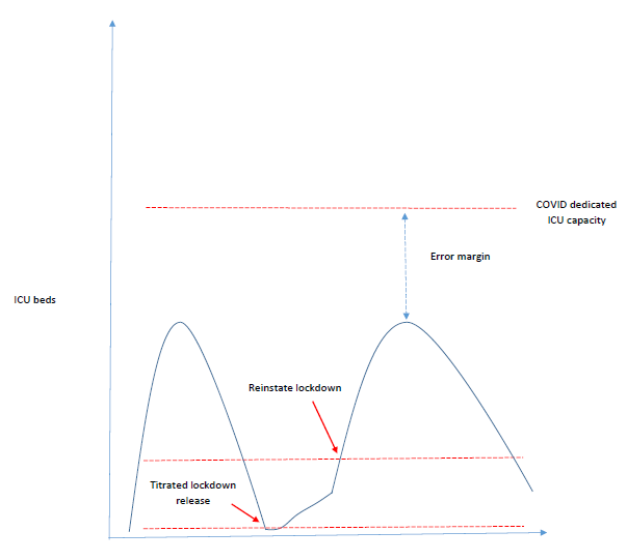
\includegraphics[width=.8\textwidth,height=5.7cm]{jpgs/lockdown_release}

  \be
  \i Implementing these cycles may be necessary to manage future outbreaks
  \i We need tools to more accurately predict
    \be \i Titrated lockdown release and Reinstate lockdown thresholds \ee 
  \ee
\end{wideframe} 




\begin{wideframe}
  \frametitle{WhatsApp based Symptom Tracker (WaSyT)} 

  \be
  \i Dedicate WhatsApp enabled phone numbers: WhatsApp Robots (WaBots)
  \be \i Similar to the World Health Organization information WhatsApp bot
      \i We only need the receiving end
      \ee 
  \i Automate receiving text and voice messages through WaBots
  \be \i The messages get decoded and saved into a database
      \i The database entries relate users, locations and symptoms across time
      \ee
  \i Analyze symptom evolution across areas and recommend interventions
  \ee
\end{wideframe} 

\begin{wideframe}
  \frametitle{WHO - COVID 19 WhatsApp Robot} 
  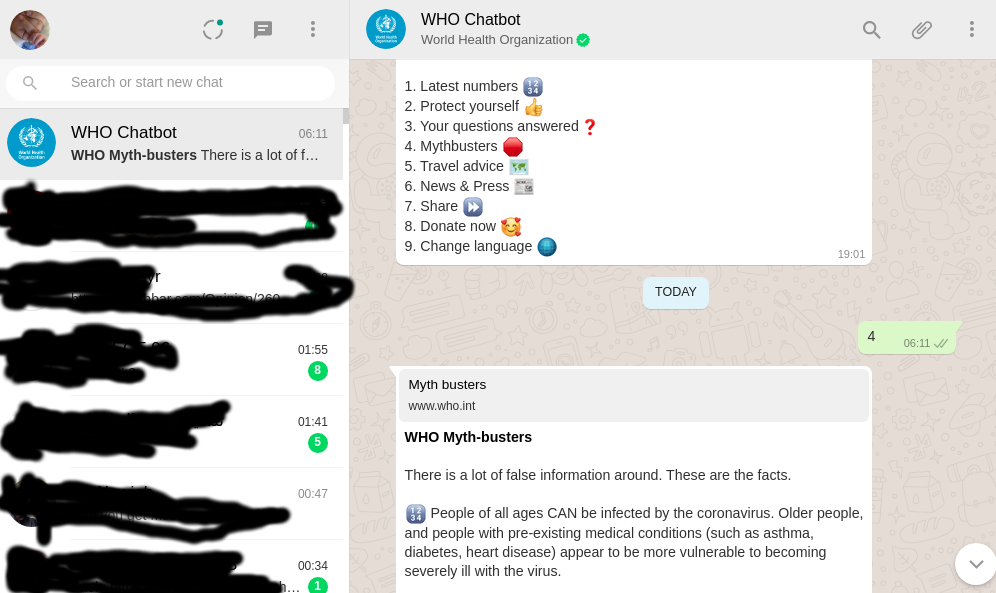
\includegraphics[width=.8\textwidth,height=5.7cm]{jpgs/WHO_Bot} 
  
  {\tiny
  \url{https://www.undp.org/content/undp/en/home/news-centre/news/2020/COVID-19_WHO_UNICEF_UNDP_Partner_with_WhatsApp_to_Get_Real_Time_Health_Information_to_Billions_around_the_World.html} 
  } 
\end{wideframe} 

\begin{wideframe}
  \frametitle{India WhatsApp Robot} 
  \framesubtitle{ \url{https://techcrunch.com/2020/03/21/india-whatsapp-mygov-corona-helpdesk-bot/} 
  }
  \be 
  \i Awareness WhatsApp robot targeting limited internet users
  \i Targets curbing down misinformation spread
  \ee
  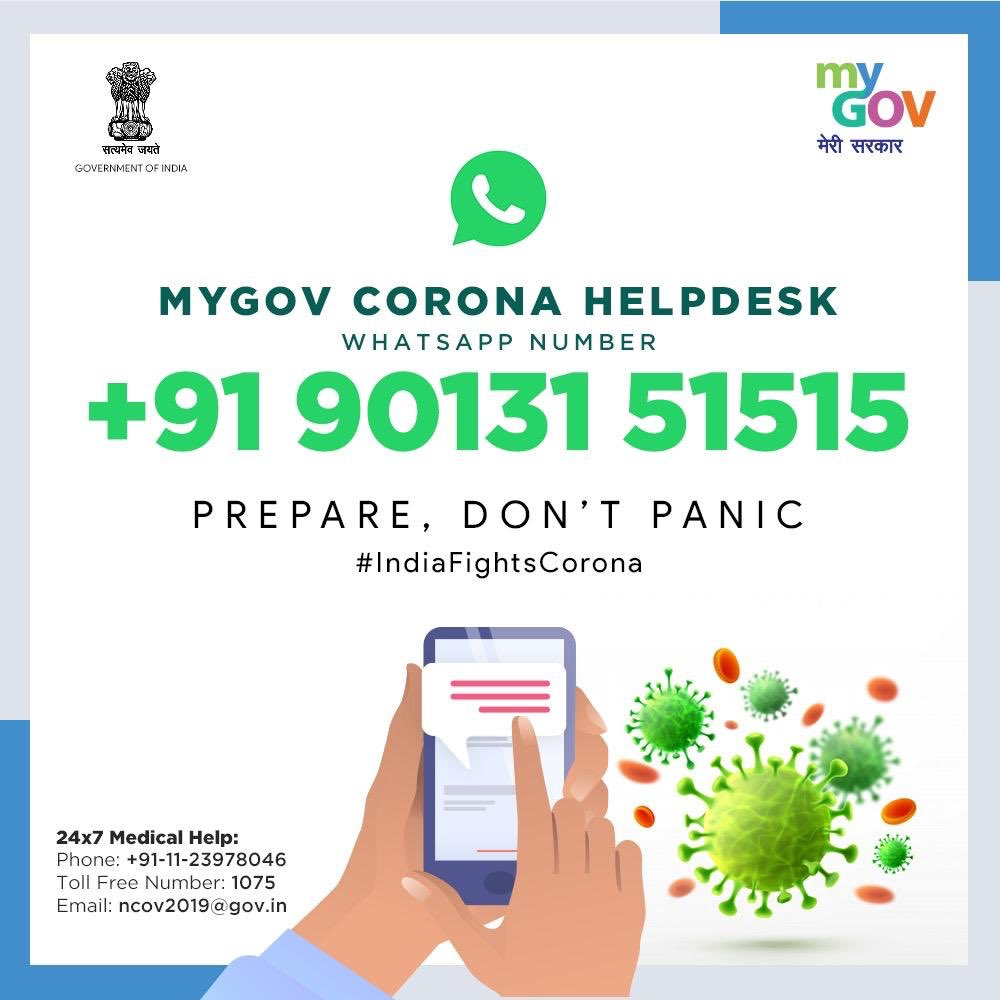
\includegraphics[width=.8\textwidth,height=5.7cm]{jpgs/ETnT2hOUEAAuoEe}
  
\end{wideframe} 



\begin{wideframe}
  \frametitle{How can this be done?}
  \be
  \i Gateway to collect messages 
    \be \i Alternative 1: WhatsApp business API
        \i Alternative 2: Chrome browser extensions over \url{web.whatsapp.com} 
    \ee
  \i Speech to text 
    \be \i Alternative 1: existing Arabic Speech recognition system 
        \be \i RDI and QCRI exist for general purpose text 
        \ee 
        \i Alternative 2: Signal processing for keyword spotting 
        \be \i More accurate but requires time for data collection and development 
        \ee
    \ee
  \i Symptom extraction from text messages 
    \be \i Natural language processing based on bag of words augmentation for each symptom
    \ee 
  \i Analytics: readily available with AUB AdHoc COVID-19 modeling team
  \ee
\end{wideframe}


\begin{wideframe}
  \frametitle{SMM-SymTrack flow diagram } 
  \input{figs/SMMSymTrak.pdf_t} 
\end{wideframe}


\begin{wideframe}
  \frametitle{What are we collecting?} 
  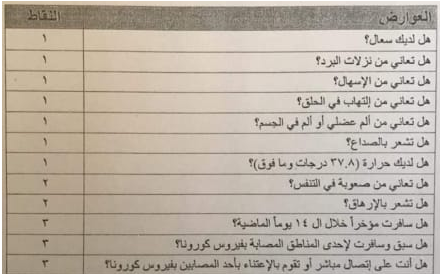
\includegraphics[width=.8\textwidth,height=5.7cm]{jpgs/symptoms} 

  Simple answers to these questions is a good start 
  (image courtesy of municipality of Intilias)
  
\end{wideframe} 

\begin{wideframe}
  \frametitle{Example messages } 
  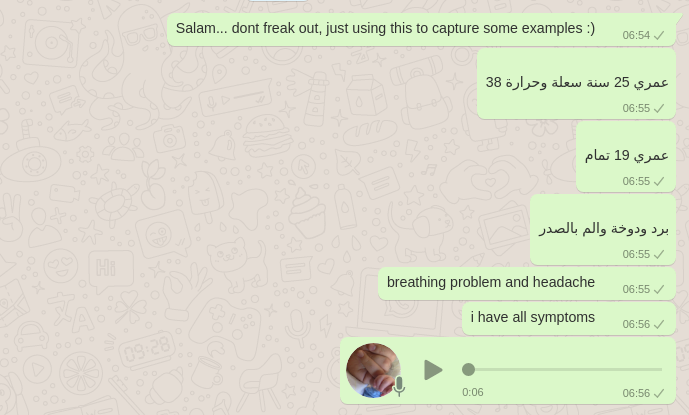
\includegraphics[width=.8\textwidth,height=5.7cm]{jpgs/examples} 

  Each message will be decoded into a database entry, 
  related to the source phone number and its location
\end{wideframe} 


\begin{wideframe}
  \frametitle{AUB-MSFEA Team} 
  \be 
  \i Nourhan Abdul-Samad, Student
  \i Ibrahim Abou-Faycal, Faculty 
  \i Christopher Haddad, Student 
  \i Ali-Akbar Haydoura, Student
  \i Hady Koteich, Student 
  \i Ayham Olleik, Student 
  \i Fadi Zaraket, Faculty 
  \ee 
\end{wideframe} 

\begin{wideframe}
  \frametitle{Status so far} 
  \be 
  \i 90\% work functional prototype
  \i Gateway is provided by \url{CM.com} and we implemented server to integrate with their API
    \be 
    \i We have two weeks free trial 
    \i Underway work to build alternative: chrome extension
    \ee
  \i Speech to text is provided by \url{RDI-ai.com} and we implemented scripts to integrate with their solution
    \be \i We have two weeks free trial 
        \i Underway work to build alternative with QCRI data set and Kaldi 
        \i May explore CMUSphinx for keyword spotting as well 
    \ee
  \i Symptom extraction from text: almost complete
  \i Integration: almost complete 
  \i Collected Arabic voice data sets of symptoms 
    \be \i 500 sentences each with Male/Female voices 
        \i Annotated at sentence level 
    \ee
  \ee 
\end{wideframe} 


\begin{wideframe}
  \frametitle{Final notes } 
  \be 
  \i Need a good tutorial and promotion campaign for people to use this once done
  \i In addition to WhatsApp, we recommend the symptom tracker to be a standalone application
  \i Do we still need to do massive testing if we do this?
  \be \i This is complementary wider scale control measure if massive testing is implemented
      \i Compensatory measure when massive testing is lacking
      \ee 
  \ee 
\end{wideframe} 


\begin{wideframe}
  \frametitle{Thank you! } 
  \be 
  \i Questions are welcome. 
  \ee 
\end{wideframe} 



\end{document}
